\subsubsection{Нет 6}
 
\zadatak Које вредности задовољавају услов
\begin{align*}
\log_2(x+1) &> \log_4x^2?
\intertext{\resenje Ако леву страну запишемо као}
2\cdot\frac12\log_2(x+1)&=\log_{2^2}(x+1)^2 
\intertext{што следи из једнакости \eqref{eq:powbase} и \eqref{eq:bpow},
добићемо}
\log_4 (x+1)^2 &> \log_4 x^2\\
(x+1)^2 &> x^2\\
x^2+2x+1&> x^2\\
2x+1&>0\\
x&>-\frac12.
\end{align*}
Како мора да важи $x>-1$ и $x\ne0$, добијамо коначно решење
$$
    x\in\ram{\left({-\frac12},0\right)\cup(0,\infty)}.    
$$
$$
\slika{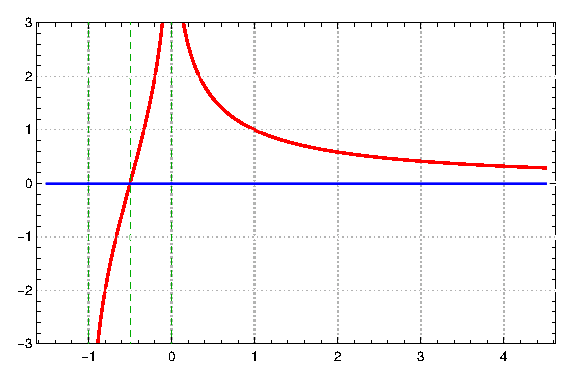
\includegraphics[width=\sirina]{eps/net6.eps}}{$y=\log_2 (x + 1)-\log_4 x^2$.}
$$

\dodatak Као што је на страни \pageref{danger} напоменуто, 
да смо $\log_4 x^2$ једноставно представили као $\log_{2^2}x^2=\log_2 x$,
добили бисмо нетачно решење. Исправно би било $\log_4 x^2=\log_2|x|$,
када бисмо посебно гледали 2 случаја: за $x>0$ и за $x<0$.
